\documentclass{mpaper}

\usepackage{minted}
\usepackage{color}
\usepackage{lmodern}
\usepackage[T1]{fontenc}
\usepackage[font=bf]{caption}
\usepackage{multirow}

\begin{document}

\title{Data-flow compilation of Fortran for FPGAs}
\author{James Macdonald}
\matricnum{2126890}

\maketitle

\begin{abstract}

FPGAs offer a low-energy alternative to GPUs and other high-performance, general purpose accelerator technologies.
They have the potential to improve code execution performance, while at the same time using less energy.
Although they have a long history of use in the electronics sector, they have traditionally required to be programmed using hardware description languages such as Verilog.  
This has stifled their adoption in high performance computing (HPC) as developing solutions for FPGA execution required expert knowledge of their operation and considerable implementation and debugging time.  
Recently, efforts have been made by the two main FPGA vendors to offer high level synthesis options by including their devices in the OpenCL standard.
While these efforts lower the barrier to entry somewhat, they still require expert knowledge and careful structuring of programs to get good performance when executing on FPGA devices. 

At the same time, there are many ageing scientific and engineering simulation code bases written in languages such as Fortran.
Many of these systems are actively used and their users would benefit from increased performance.
Rewriting these systems to target new accelerator types by hand represents a major undertaking, financially and in terms of time.
% and , for which their users neither have the time nor expertise.

This paper proposes a method of merging the potential of FPGAs and Fortran simulation systems.
We propose a refactoring compiler that enables scientists to compile their Fortran programs to produce an optimised OpenCL pipeline.
The compiler's output can be used as input to vendor specific HLS tools to generate a bitstream for execution using an FPGA.

The compiler is evaluated and shown to be able to handle a variety of real world scientific simulation code bases and produce OpenCL that has competitive resource usage and execution characteristics when compared to the same code translated by a human expert.

\end{abstract}

\section{Introduction}

Computer simulation has long been a cornerstone of cutting edge scientific and engineering work. Simulators allow scientists and engineers to test their theories and designs far more rapidly than the physical world allows.
One of the most striking examples of advanced simulation use in our everyday lives is the forecasting of extreme weather events.
The need for better predictions of environmental events such as hurricanes has always been apparent.
The death and destruction caused by these events means any increase in forecast accuracy can save a huge number of lives.
As extreme weather events become more frequent and severe due to climate change, the need for high-resolution forecasts is at an all time high.

Simulation systems often comprise of performing the same series of operations on many points, over many time steps.
This means they are computationally intensive and not bound by other bottlenecks such as I/O, this makes them ideal candidates for optimisation.
Many of the computer models used for simulation tasks are legacy systems, often written in languages such as Fortran.
% Though these models maybe classed as legacy in terms of software engineering, they are battle-tested and are known to provide accurate results.
In addition to these legacy models, many new models are being developed by scientists who still use Fortran.
As a language, Fortran provides a number of primitives that are useful for scientific code, while also being familiar to scientists who have other priorities other than learning new languages and cutting edge computer science techniques.

Field Programmable Gate Arrays (FPGAs) provide an exciting new avenue in the world of HPC.
Results show they can offer huge performance increases, while also drastically reducing energy consumption \cite{Vanderbauwhede2014,Prasanna2006,Dimond2011}.
FPGAs have long been a feature of hardware development work flows and working with them required expert knowledge of hardware description languages such as Verilog or VHDL.
Recently, efforts have been made to open up access to FPGAs by integrating them with the OpenCL parallel programming framework.
Although this lowers the bar to entry significantly, it still requires expertise and careful structuring of programs in order to take full advantage of execution on an FPGA.

When these factors are considered together it becomes clear that novel ways of marrying up the power of FPGAs with the wealth of Fortran simulation codes would be extremely beneficial.
If a turn-key solution for porting these simulators to FPGAs was available, scientists would be able to run faster, higher-accuracy simulations, while reducing energy usage with next to no additional effort on their part.

This paper presents a \textit{refactoring compiler} than analyses scientific simulation code written in Fortran and outputs refactored Fortran that is suitable for high performance execution using FPGA devices. The process outlined in this paper requires no changes to be made to the input source.

%%%%%%%%%%%%%%%%%%%%%%%%%%%%%%%%%%%%%%%%%%%%%%%%%%%%%%%%%%%%%%%%%%%
\subsection{Problem Statement and Aims}

This aim of this work is to create a compiler capable of compiling Fortran scientific simulation codes to OpenCL optimised for execution on FPGA devices.

The output from this compiler will be a Fortran OpenCL dialect that can be converted to standard OpenCL C using an existing compiler \cite{VanderbauwhedeDavidson2018}.
The output from this existing compiler can then be used as input to the FPGA vendor's HLS flow \cite{IntelCorporation, Xilinx}.
The HLS flow will then produce a bitstream that can be executed by the FPGA.

If successful, this project will significantly reduce the burden associated with porting legacy Fortran simulators such as the 2D Shallow Water Model \cite{Hall2009} and the Large Eddy Simulator for Urban Flows \cite{Nakayama2011} for acceleration using FPGAs.
This could potentially unlock huge increases in performance with minimal manual effort.

%%%%%%%%%%%%%%%%%%%%%%%%%%%%%%%%%%%%%%%%%%%%%%%%%%%%%%%%%%%%%%%%%%%
\section{Background Survey}

This work comes from a series of efforts towards developing tooling that allows battle-tested software, often developed decades ago, to be run on the latest hardware.
It builds on research from the HPC community at large \cite{Vanderbauwhede2014, Dimond2011, Corrigan2012, Oancea2012, Prasanna2006, Holewinski2012} but also from specific works produced from within the computer science department at the University of Glasgow in particular \cite{Vanderbauwhede2012, Nabi2015, Davidson2016, VanderbauwhedeNabi2018, VanderbauwhedeDavidson2018}.

\subsection{Fortran Refactoring}

Fortran has always been popular with the scientific community and continues to be so today  \cite{VanderbauwhedeDavidson2018}.
As such, there have been many attempts \cite{Oancea2012, Corrigan2012, Orchard2013, Overbey2005} to create automated refactorings to improve execution performance and aid maintainability. 

Corrigan and L{\"{o}}hner proposed a system to allow the FEFLO CFD simulator \cite{Lbhner2001} to be ported for execution on GPUs via CUDA and the Thrust library \cite{Library}.
The compiler is developed in Python, and is specifically designed to work with the FEFLO codebase.
OpenMP \cite{OpenMP} annotations present in the FEFLO code are used by the compiler to output CUDA kernels.
The authors make it clear they have not developed a general purpose auto-parallelizing compiler.
They state the main goal of the work is to allow the FEFLO developers to continue developing in Fortran, while allowing users of the simulator to take advantage of modern GPU hardware.
The authors acknowledge that this limits the overall contribution from their work.
As the compiler is only designed to work with one codebase the authors discuss heuristics that are used as part of its operation.
Reliance on FEFLO specific heuristics means it is likely to be difficult to extend the compiler to work with other projects in the future.
One final issue with the work is that it relies heavily on the Thrust library which is CUDA specific and thus only supported on NVIDIA hardware.
This significantly limits the range of GPUs that the ported code can be used with, and therefore the number of end users that may benefit from the work.

One of the papers most influential to the direction of this work is ``Domain-specific acceleration and auto-parallelization of legacy scientific code in Fortran 77 using source-to-source compilation''\cite{VanderbauwhedeDavidson2018}. 
The authors present a three-phase compiler, that takes Fortran 77 code as input and outputs OpenCL code optimised for execution using a GPU.
The first phase of the multi-stage compiler cleans up and converts Fortran 77 code to Fortran 95.
It searches for and corrects potentially problematic coding practices allowed in Fortran 77.
For example, the compiler ensures subroutine parameters are annotated with \texttt{intent} statements, adding them where they are missing, and removes any \texttt{common} blocks from the input source.
This makes the flow of the program more obvious and easier for parallelization refactorings to be applied during the next phase of compilation.
The compiler is also used in the final stage of the compilation process to convert the Fortran-syntax OpenCL device code produced by the refactoring compiler to standard OpenCL C that can be compiled to execute on a GPU.

\subsection{High-level functions, identifying parallelism}

Identifying and expressing parallelism at a high level is central to this project.
``Financial software on GPUs'' \cite{Oancea2012} provides a good overview of how functional programming and higher-order functions can be used to explicitly represent parallelism.
The paper shows how map and reduce operations can be parallelised while still remaining provably correct.
The work focuses on optimising Monte-Carlo simulation algorithms often used for financial forecasting tasks.
Contrasting Fortran and Haskell code samples are used to show how the functional style of Haskell allows parallelism to be made obvious, whereas the imperative style of Fortran code can obfuscate an algorithm's inherent parallelism.

The refactoring compiler presented in \cite{VanderbauwhedeDavidson2018} is only one of the paper's contributions. 
There are multiple compile stages involved in getting the Fortran code ready to be executed on a GPU.
The second compiler in the paper analyses the output from the Fortran 77 \textrightarrow Fortran 95 compiler and attempts to parallelizes it.
The compiler looks for map and reduce patterns in the Fortran source and converts these to OpenCL kernels which perform the same computation.
The analysis is fully automated and does not require any modifications to be made to the Fortran input.


\subsection{OpenCL Programming for FPGAs}
\label{FPGA_OpenCL}

OpenCL is a data parallel programming API that allows users to take advantage of accelerator hardware. 
Traditionally this meant allowing users to perform computations using their Graphics Programming Units (GPU) which normally were only used for gaming.
OpenCL execution is divided between the ``host'' (usually the main CPU of the system) and the ``device'' (the accelerator device that executes the main workload e.g. CPU, GPU or FPGA).
OpenCL exposes a tiered memory model, allowing developers to designate whether data should be stored in global, local or private memory.
Where data is stored on the device is an implementation detail and varies between devices/vendors.

As OpenCL originally targeted GPUs it offered a data parallel execution style, allowing the user to write functions (or ``kernels'' in OpenCL terminology) that are executed over all the data points in the input.
This has the same net effect as sequential iteration inside a loop construct over the input array.  
This allows loops to be replaced by using OpenCL API calls to execute kernels over the same range of data.  

When writing OpenCL kernels for GPUs, where data is stored in the memory hierarchy is important, as it can affect what data kernels can access.
However, it is of less concern than for devices such as FPGAs.
The global memory of a GPU tends to be clocked at a very high speed and consequently has very low access latency.
This means global memory can be accessed from within kernels without negatively effecting performance. 

Kernels are written in a subset of the C language called OpenCL C, the syntax is very similar to C but missing some features like recursion and dynamic memory allocation, and with some additionally OpenCL added.
The host is responsible for performing any set up required (e.g. passing arguments to the kernels) as well as retrieving any results calculated on the device, while the device carries out the brunt of the work.
If the programmer wants to run multiple kernels on the input then they queue them up one after another from the host.

An FPGA is a programmable logic device that allows the programmer to lay the instructions they want to perform out in a pipeline on the chip.
FPGAs are made up of DSP units, block RAMs, lookup tables and programmable interconnect which can be used to connect the other components. 
Traditionally FPGAs could only be programmed using hardware description languages but recently there has been a push from the two main vendors (Intel and Xilinx \cite{IntelCorporation, Xilinx}) to incorporate their FPGAs with the OpenCL framework.
FPGA programming with OpenCL requires different mental models than can be used when OpenCL is used to program GPUs.
For example, accesses from kernels to the global memory of an FPGA are prohibitively expensive and cannot be performed without ruining overall performance.
To minimise the number of reads from global memory a pipeline must be formed, at the beginning of which data is read from global memory and only written back to global memory at the end.
To build a pipeline, kernels are linked with a new OpenCL C primitive called pipes.
Kernel's can read and write to a pipe allowing multiple data items to be processed at different stages of the pipeline at once.
Pipes have a configurable capacity, that sets how many items can be written to them without being read out.
Once a pipe reaches its capacity additional calls to write to it will block halting execution of the kernel containing the call.
Similarly if a pipe is empty, any calls to read it will block.
The default capacity varies between between vendor implementations of the OpenCL specification, therefore it is safest to assume that reads and writes must be perfectly matched to prevent deadlock and to ensure all data items are processed by all stages of the pipeline. 

Due to the asynchronous nature of an FPGA pipeline, all the kernels are launched at once instead of each being queued for execution over the whole data input one by one.
Due to this different mode of operation a driver loop needs to be inserted into the device kernels to drive the pipeline and ensure all data items pass through the pipeline.
The size of this driver loop has to be large enough to cover all the data items that the pipeline is to process.
For example, if in a sequential version of program a 3D array is accessed using 3 nested loops, each looping over one of the array's dimensions, the driver loop range will equal the product of the 3 original loop's ranges. 

After version 2.0 of the OpenCL standard was released introducing the ability to program FPGAs using pipes, many papers were released which explored how they performed.
In their 2016 paper \cite{Momeni2016} the authors provide a detailed explanation of the new architecture that must be used to unlock the potential of FPGAs, along with a breakdown of the performance they managed to achieve when they implemented an image analysis pipeline.
Another paper that emphasises the importance of exploiting pipeline parallelism to unlock the full potential of an FPGA, was published by Vanderbauwhede and Nabi in 2018 \cite{VanderbauwhedeNabi2018}.
The authors explain why reading from and writing to global is so expensive on FPGAs and provide a detailed analysis of how to restructure device code to allow it to run well on FPGAs.

\subsection{Stencil computations and implication for FPGAs}
\label{stencil_computations}

\begin{figure}
    \centering
    
\includegraphics[scale=0.5]{images/stencil.png}
    \caption{Example of stencil calculation}
    \label{fig:stencil}
\end{figure}

Stencil computations are often central to the operation of much simulation software. 
A stencil computation occurs when processing an array of values.
To perform a stencil computation and update the value of an array element the current value of one or more adjacent elements is required, as opposed to only the current value of that element.
Figure \ref{fig:stencil} illustrates the dependencies (depicted with red arrows) of the central point to the points around it. 
Due to their prevalence in simulation codes much work has been carried out to optimise stencil computations in order to improve simulation performance. 

The key to optimising stencil codes is reducing expensive memory access operations. 
Therefore work optimising them normally focuses on optimising their operation on one particular class of device. 
Stencil optimisation efforts have typically targeted GPUs as traditionally they have been more widely used.
One example targeting GPUs is found in the paper ``High-performance code generation for stencil computations on GPU architectures'' \cite{Holewinski2012}.
The authors present a framework that can generate efficient stencil code that can be executed using GPUs. 
The framework operates by increasing the computational workload on the GPU in order to reduce the required memory bandwidth.
This trade-off was found to be beneficial and offer improved performance. 

While optimising stencil memory accesses on GPUs is important, it is essential when running them on FPGAs.
GPUs benefit from high speed, low-latency memories that operate at high enough clock speeds to make random memory accesses possible without having an overly adverse effect on performance. 
However, accesses to an FPGAs global memory is a ``performance killer'' and leads to far below optimal performance.
To achieve good performance on an FPGA the fast on-chip block RAM buffers need to be utilised. 
These buffers are limited in their capacity and therefore cannot be used to hold all the data that may be being processed by the kernels currently executing on an FPGA. 
This means that intelligent ways need to be found of buffering data on-chip when executing stencil computations using an FPGA.

Many papers describing porting stencil code to FPGAs encounter the situation laid out above and arrive at a similar conclusion to solve it.
Fu and Clapp in their 2011 paper \cite{Fu2011} describe how they solved the global memory access problem when implementing the 3D Reverse Time Migration algorithm using FPGAs as the hardware platform.
They make reference to using the FPGA's block RAMs to store a ``window of the input stream'' allowing adjacent stencil locations to be accessed without accessing the main memory which would lead to sub par performance.
Waidyasooriya et al. \cite{Waidyasooriya2017} describe an OpenCL based framework that aims to make it easy to construct optimised stencil based code that run efficiently on FPGAs.
They propose ``pipelined computation modules'' in which each module is responsible for buffering the data items required to perform a stencil computation and then using the buffered data to carry out the stencil computation itself.

The approach adopted in this work is inspired by the ``smart cache'' system laid out by Vanderbauwhede and Nabi in their 2018 paper \cite{VanderbauwhedeNabi2018}.
In their paper they describe hand translating the 2D Shallow Water Model \cite{Hall2009} for execution on FPGAs. 
Because the 2D Shallow Water Model makes use of stencils they identify the same memory bandwidth problem as identified in the papers \cite{Fu2011,Waidyasooriya2017}.
To combat this problem they propose constructing a computation pipeline with smart caches before any computation kernels which access an array via a stencil.
A smart cache is formed by analysing all the points that make up a stencil. 
The number of values that the smart cache needs to buffer can then be calculated.
This allows the smart cache to produce output streams for all the individual points that form the stencil.
Figure \ref{fig:smartcache} provides a high level overview of how a smart cache works and a more detailed explanation of how they are generated can be found in Section \ref{data_flow_analysis_and_support_kernel_generation}.

\begin{figure}
    \centering
    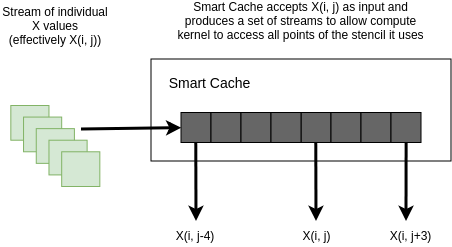
\includegraphics[scale=0.5]{images/Smart_Cache_Buffer.png}
    \caption{High level overview of smart cache operation}
    \label{fig:smartcache}
\end{figure}

\section{Compiler Architecture}

The refactoring compiler that forms the main research output of this project is designed to translate a Fortran input program to an Fortran OpenCL host program and a Fortran-dialect OpenCL device module. The compiler is designed to work in tandem with the RF4A compiler, also developed at the University of Glasgow and presented in \cite{VanderbauwhedeDavidson2018, VanderbauwhedeNabi2018}. The compiler developed during this work accepts as its input the output from the RF4A compiler and then has the device portion of its output converted from Fortran dialect OpenCL to standard OpenCL C. 

The compiler presented here (named F4) is developed in Haskell and makes extensive usage of the \textit{Data.Generics} package and the \textit{'scrap your boilerplate'} style of programming that it enables. The compiler is structured as a series of passes over the input source. Two of the passes used in F4 are borrowed from the AutoParallel-Fortran (AP-F) compiler also presented in \cite{VanderbauwhedeDavidson2018}, AP-F has a similar goal to F4 however it targets GPU devices.  

The compiler implementation proposed in this work has 5 main stages as depicted in Figure \ref{compilation_flow}.
Each stage is discussed in detail below. 

\begin{figure*}
\begin{center}
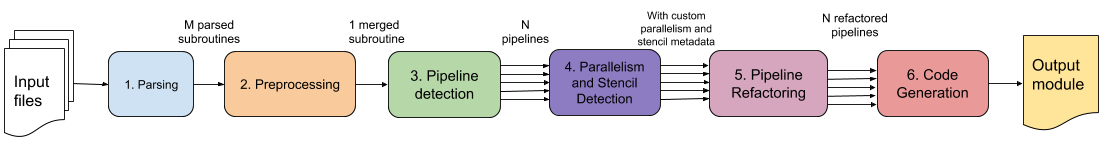
\includegraphics[scale=0.45]{images/Compilation_flow.png}
\end{center}
\caption{\label{compilation_flow}High-level overview of F4's compilation stages and the data that passes between them}
\end{figure*}

\subsection{Parsing}
\label{parsing}

Developing a parser for a language as vast and varied as Fortran from scratch is a major undertaking, and would have significantly eaten into the development time available for more impactful and interesting areas of the project.
The AP-F project faced exactly the same challenge.
As this project used two of the analysis passes from AP-F the parsed abstract syntax tree (AST) needed to be compatible.
Therefore the decision was made to use the Haskell \textit{language-fortran}\footnote{http://hackage.haskell.org/package/language-fortran} package, with the modifications made to it as part of the AP-F project.
This choice enabled a triple benefit: 
\begin{itemize}
    \item A Fortran parser did not need to be developed;
    \item Tried and tested analysis passes from the AP-F project could be reused in this project;
    \item Bugs that were found in the \textit{language-fortran} implementation and mitigated using a custom preprocessor as part of AP-F would not have to be re-debugged as part of F4's development.  
\end{itemize}

\subsubsection*{Source File Structure + Preprocessing}

As AP-F and F4 are designed to work in conjunction with RF4A, they both expect the input files they are processing to have a certain structure.
They expect a series of Fortran 95 files, each containing one subroutine per file (with the filename matching the subroutine name), and one main file which acts as the program's entry point containing calls to the other subroutines.
As this is what RF4A is designed to produce both refactoring compilers can be designed to work in line with these assumptions. 

Before parsing with \textit{language-fortran} AP-F used a custom preprocessor to sanitise its input files. 
The preprocessor includes some custom rules designed to minimise the effect of any divergence between the input accepted by \textit{language-fortran} and a standard Fortran compiler such as \texttt{gfortran}\footnote{https://gcc.gnu.org/wiki/GFortran}. 
This largely revolves around superficial aspects of the code, such as how \textit{language-fortran} handles white space and the fact that Fortran is case insensitive. 
The custom preprocessor operates by performing a series of simple find and replace operations on the input.
In order to benefit from the debugging effort expended developing the preprocessor, it is also used in this project.

% As well as producing an AST representing the contents of the parsed file, the parser also builds an argument translation table for each call statement contained in the subroutine. The argument translation table maps the names of the variables used as arguments in a call statement to the parameter names they are being passed into. The set of AST/argument translation table pairs are then passed to the next stage of the compilation pipeline.

\subsubsection*{Language-Fortran}

The preprocessed source is then parsed using \textit{language-fortran}.
\textit{language-fortran} is an open source Fortran parser developed by Jason Dagit, with its source made available through GitHub\footnote{https://github.com/dagit/language-Fortran}.
The licence used to distribute \textit{language-fortran} allows modification when the stipulated conditions are met - AP-F and F4 both meet the conditions.
As modifications were necessary to allow \textit{language-fortran} to be used as part of this project the final version can be found in the project repository. 

\textit{language-fortran} is based on the \texttt{happy} and \texttt{alex}, parser and lexer generator system.
\texttt{alex} allows users to specify a Lexer.x file in a Haskell-like syntax which is then compiled to produce a Haskell module implementing the lexer.
The lexer produces a token stream that can then be fed as the input to a parser generated by \texttt{happy}. 

\texttt{happy} is responsible for parser generation and again uses a Haskell-like input syntax to define a series of production rules. 
Each production rule allows the user to construct one of a series of user defined Haskell data types and populate it with appropriate values output during the parsing process.
Similarly to \texttt{alex}, \texttt{happy} accepts an input file which contains a Haskell-like syntax for defining production rules and both non-terminal and terminal symbols.
\texttt{happy} outputs a pure Haskell version of the input specification allowing the user to use the parser from any Haskell program. 

The final key element of the parser apparatus is the file defining the AST produced by the parser and all the nodes that make it up.
These data types are defined as pure Haskell in the \texttt{Fortran.hs} file that comes as part of the \textit{language-fortran} project.
One of the most important customisations made to the \textit{language-fortran} package as part of the AP-F project was to add two custom node types to the AST.
Custom \texttt{OpenCLMap} or \texttt{OpenCLReduce} nodes are used to replace Fortran loops and identify them as either a map or a reduce.

This project required similar functionality on top of what existed already.
To facilitate the stencil detection pass of the compiler (described in Section \ref{pipeline_refactoring}) the \texttt{OpenCLStencil} constructor was added to the existing \texttt{Fortran} statement type.
Two new types \texttt{Stencil} and \texttt{StencilIndex} were added to allow stencil metadata to be attached to the AST. 
This made it easy for later compilation passes to access the data.

% One other constructor was added to the \texttt{Fortran} type named \texttt{OriginalSubContainer}.
% This constructor was designed to encapsulate a block of code along with a name specifying the subroutine that the code originally came from.
% This proved very useful at various stages of the pipeline allow subroutines to merged and split at will while not loosing track of where blocks of code had come form originally.

All the additions made to the \texttt{Fortran} type are custom metadata used by the AP-F and F4 projects and do not relate to any real Fortran language features.
The pretty printer used as part of this project outputs the custom metadata types as comments to aid debugging while keeping the output syntactically valid.
The listings later in this paper provide examples of this output.

Two bugs were also identified in the parser that affect this project but not the AP-F project. 
The first bug led to the parser skipping any line that begun with a \texttt{C} as this is Fortran 77 syntax for a multi-line comment.
The mitigation for this was simply to remove the tokenization rule that handled Fortran 77 comments from the \texttt{Lexer.x} file.
This can be done safely in the knowledge that the input to the F4 compiler is always going to come from the RF4A compiler.
RF4A is designed to refactor Fortran 77 code to Fortran 95 to simplify later processing.
This means any comments beginning with \texttt{C} will have been replaced with ones beginning with \texttt{!} as is standard in Fortran 95.

The second bug caused the parser to ignore parenthesises when it encountered them as part of a larger expression.
This meant the code in the AST did not always follow the same precedence rules as the input code and if executed, would produce different results.
To fix this a new \texttt{ParenthesizedExpr} constructor was added to the \texttt{Expr} data type in the \texttt{Fortran.hs} AST definition file and the expression production rule in the \texttt{Parser.y} file was updated to use the newly added constructor. 

The effect of these bugs was isolated to this project and did not affect AP-F because of the approach it took to code generation.
The output from the AP-F project was based as far as possible on the exact source lines that were fed to it as input.
This involved storing input source lines as strings alongside the parsed AST. 
Then, when it came to code generation, sections of code were emitted directly from the cached input lines unless they had been generated by the AP-F compiler.
This approach was feasible for the AP-F project because the compiler only needed to add code on to support execution on GPUs. 
As this project targets FPGAs, the compiler must not only add significantly more code but also rewrite almost every single line of existing code.
This means there would be little point storing the original source lines for emission in the code gen-stage.
Therefore, a more traditional approach to code generation was adopted and code was emitted by walking the AST with a pretty printer.
If the parenthesises were omitted from the AST during parsing the code emitted by the pretty printer would be incorrect.
The bug which caused lines beginning with \texttt{C} to be discarded by the parser did not affect AP-F because it emitted most of its output directly from its input line cache which still contained any lines beginning with \texttt{C}.
Any other lines that made up the output were directly generated by the compiler itself so would not be affected by the bug.

\subsubsection*{Argument Translation Parsing}

As well as producing an AST representing the contents of the parsed file, the parser also builds an argument translation table for each call statement contained in a subroutine. The argument translation table maps the names of the variables used as arguments in a call statement to the parameter names they are being passed into. The set of AST/argument translation table pairs are then passed to the next stage of the compilation pipeline.

\subsection{Preprocessing Passes}

With the results of the parsing phase, two preprocessing passes are executed in order to prepare the Fortran for the main analysis and refactoring passes used by the compiler. 

\subsubsection*{Stencil Constant Removal}
\label{stencil_constant_removal}

If an array is to be processed in a streaming fashion (as is required for good performance when using an FPGA) it must be accessed within a loop, using the loop indices.
The loop indices can be used directly or with simple integer offsets applied to them.
If an array access contains constants (as shown in Listing \ref{lst:stencil_constant_removal}) it will not be able to be streamed.
To mitigate this, a series of rewrite rules were introduced to convert any array accesses using constants to equivalent code without any.

The first step in the rewrite is to add an extra loop to the loop nest so that its loop  variable can be used as the an array index in place of the constant.
To decide the range over which the inserted loop will iterate, the declaration of array accessed using a constant index is examined.
The values present for the array's upper and lower index bound for the appropriate dimension are used as loop bounds.
Next, the nesting direction of the existing loop nest must be inferred.
To do this the nesting order of the loop nests is compared to the usage order of their loop variables in the array access in question.
A loop nest can have normal, reversed, either or unknown ordering.
F4 can handle normal, reversed or either ordering.
When it encounters unknown ordering it is unable to determine at what nest level to insert the generated loop.
This means it cannot remove the constant from the stencil computation and therefore aborts compilation with an error.
Based on the position of the constant index in the array accesses, and the nesting order of the loop nest, the synthesised loop is inserted at the appropriate nest level.


Next, the constants are substituted for the loop index plus the original constant value to produce the intermediary form show in Listing \ref{lst:stencil_constant_removal}.

Finally, the code is refactored to remove any array assignments that contain an offset index on the left hand side, as this would not be able to be analysed during later stages of compilation.
The refactor works by determining the offset that is applied to the LHS array access, negating it and adding this to indices on both sides of the assignment (leading to zero on the LHS, meaning there is no offset). 
Lastly, a guard is added so that the statement only executes when the synthetic loop index is equal to the original LHS constant value, thus ensuring the code still operates as it did before the rewrite. 

\subsubsection*{Subroutine Merging}

After any constants have been removed from the stencil accesses, the subroutines which were specified at the command line for offload to the FPGA are merged together to form one coherent\footnote{All references to a named symbol refer to the same thing.} subroutine.

To do, this the argument translation table referring to calls made in the main subroutine is used.
In each of the offload subroutines all occurrences of variables present in its parameter list are replaced with the matching variable from the main subroutine. 
This mapping is determined based on the argument translation table.
This process could lead to variable name conflicts as there may be existing local variables declared that have the same name as the arguments passed to any of the other subroutines from the main method.
To prevent conflicts such as this, after performing the substitution, the compiler checks for conflicts and if it detects any it appends \texttt{\_F4\_CAS} to all occurrences of the argument variable it finds in the main subroutine.
It then updates the argument translation table, and retries the substitution.
This process repeats until no conflicts exist. 

Once the parameter name $\rightarrow$ argument name substitution is complete all the offload subroutine bodies are concatenated. 
The offload subroutines declaration and parameter lists can also be concatenated.
Distinct items from both of the concatenated results are selected. 
The new lists are then combined with the merged subroutine bodies to form one coherent block of code with all the appropriate declarations and parameters present, ready to be operated on by the rest of the compilation pipeline.

\subsection{Pipeline Detection}
\label{pipeline_detection}

The goal of the pipeline detection phase is to split the previously merged offload subroutine into chunks in which all the loop nests complete a similar number of iterations. 
The analysis works by counting the number of loops present in each loop nest and grouping them with adjacent loop nests where the same number of loops are present.

A pipeline represents a block of execution that the FPGA can execute.
Later in the compilation process additional logic is inserted to facilitate reading values from the FPGA's main memory, and streaming them into a pipeline, as well as logic to write back updated values to main memory once a pipeline has completed execution.
By treating each pipeline as an isolated execution context, multiple pipelines can be executed one after another. 
Once all the pipelines that an offload subroutine has been separated into have been executed, it is equivalent to the merged offload routine being executed in its entirety.

As explained in Section \ref{FPGA_OpenCL}, an FPGA pipeline written in OpenCL must have a driver loop that drives the pipe accesses and ensure all data items pass through all processing steps. 
Section \ref{FPGA_OpenCL} also highlighted that the number of pipe read/write operations on a pipe must be exactly matched to prevent deadlocks. 
These two requirements mean that the driver loop used within a pipeline must iterate over the range of the largest stream within that pipeline.
Within one merged subroutine it is perfectly possible that there are streams of vastly different sizes, but larger streams are only active in selected sections of the pipeline.
If only one pipeline was created that shared a common driver loop all sections of the pipeline would have to perform the maximum number of iterations, even though many sections of it perform no processing over a large chunk of the driver loop iteration range. 
Therefore, by splitting the merged offload subroutine into pipeline subroutines we prevent wasting many processing cycles on the FPGA. 
The merged offload subroutine is split using a heuristic. 
Contiguous sections with loop nests of the same depth should be separated into individual pipelines. 

The result of the pipeline detection phase is $N$ pipeline subroutines.
Each of the pipeline subroutines contains the appropriate section of the merged offload subroutine body, plus any supporting declarations and arguments.

\subsection{Parallelism and Stencil Detection}
\label{parallelism_and_stencil_detection}

In order to make the transformations necessary to the code, data must first be gathered to be used as input. 
The stencil and map/reduce detection passes attach their results to the AST directly, making it easier to find the relevant code at later stages of the compilation pipeline.

The first analysis to run is the map and reduce detection pass.
This pass was developed as part of the AP-F project and has been used unchanged.
The goal of the pass is to identify whether a loop represents a map or a reduce.
It does this by analysing array accesses and variable writes within the loop.
If all the array accesses within a loop make use of all the loop index variables and none of the variable writes form a loop carry dependency\footnote{A loop carry dependency occurs when the a memory location is written multiple times during the iteration of a loop.}, that loop is designated as representing a map and the loop node in the AST is replaced by an \texttt{OpenCLMap} node. 
The inserted \texttt{OpenCLMap} node contains: the name of the loop index variable, the range over which the loop operated, and the body of the loop.
Attaching the data to the AST in this way allows later analysis to make use of them.
Reduction detection works in the same way as map detection.
However, it doesn't have the requirement of no loop carry dependencies being present.
This time an \texttt{OpenCLReduce} node is used to replace the original loop node in the AST.
The node contains the same information as the \texttt{OpenCLMap} node, along with one extra field - a list of the names of the reduction variables that are calculated by the loop.

After the map/reduce detection pass, a newly implemented stencil detection pass is executed. 
The stencil detection pass inspects all the bodies of the newly created \texttt{OpenCLMap}/ \texttt{OpenCLReduce} nests, looking for array accesses. 
The analysis inspects all array accesses (both reads and writes), first checking that they all make consistent use of the relevant loop variables, indicated by the \texttt{OpenCLMap} or \texttt{OpenCLReduce} nodes.
Array accesses are deemed to be consistent if the same loop variables are always used in the same index position when accessing the same array within the body of a map/reduce nest. 
Once all the array accesses have been validated, the stencil detection algorithm examines the expressions that make up the indices in each array access to determine whether or not the loop variable has a constant offset applied to it or not.
If a block contains multiple accesses to the same array using different stencil offsets then it forms a stencil as described in Section \ref{stencil_computations}.
If stencil accesses are found within a map/reduce nest body an \texttt{OpenCLStencil} node is produced to encapsulate it and store information about the stencils.

The information is stored in a list of \texttt{Stencil} items - one for each array accessed via a stencil. 
Each \texttt{Stencil} item contains the name of the array that the stencil is applied to, a list stencil points, the dimensionality of the array, and the number of points that make up the stencil.
Listing \ref{lst:stencil_detection} shows an example of the output from the stencil detection pass.
Here we can see a stencil has been detected on the \texttt{eta} array.
The stencil consists of 3 points \texttt{(1,0)}, \texttt{(0,0)}, \texttt{(0,1)} representing the three distinct accesses (\texttt{eta(j+1,k)}, \texttt{eta(j,k)} and \texttt{eta(j,k+1)}) respectively.


After the stencil detection process is complete another pass from the AP-F compiler is executed.
This pass aims to fuse together as many nested or adjacent map/reduce nodes as possible.
The criteria for fusing nested loops is that the body of the outer \texttt{OpenCLMap} or \texttt{OpenCLReduce} only contains one statement, and this statement is of the same type as the enclosing statement (e.g. a nest of only \texttt{OpenCLMap} nodes or a nest of only \texttt{OpenCLReduce} nodes).
Next, the compiler attempts to merge adjacent map or reduce nodes.
A pair of adjacent maps/reduces is defined as, two nodes of the same type appearing in the source code directly one after another, with no intervening statements.
To merge adjacent loops the following criteria must be met: the loop index names must match, the loop indices must start at the same value, the loop end values must only differ by an a specified threshold, and finally, by fusing two adjacent loops the compiler must not introduce a loop carry dependency. 

While this pass provided some performance benefit when used as part of AP-F (due to reducing the number of output OpenCL device kernels that need to be launched), it does not provide such a benefit to code executing on an FPGA, as all the kernels that make up a pipeline execute in parallel. 
The compilation pass is used in this compiler because it consolidates the AST, drastically thinning the numbers of \texttt{OpenCLMap} and \texttt{OpenCLReduce} nodes, and makes processing at later stages easier.  

The behaviour of the loop fusion pass highlights why during the stencil detection phase the \texttt{OpenCLStencil} node is attached to the AST encapsulating existing map/reduce nests.
By attaching the stencil node to the AST in this way, F4 prevents the aggressive loop fusion (that can be applied to code destined for GPU execution) producing output code with far fewer OpenCL kernels.
However, these kernels will make accesses to global memory.
This illustrates one of the most fundamental differences between code targeted for GPUs and code targeted at FPGAs. 
As discussed in Section \ref{FPGA_OpenCL}, accesses to global memory handicap the performance of an FPGA and therefore F4 must insert smart caches between kernels that AP-F could have merged.


\subsection{Pipeline Refactoring Passes}
\label{pipeline_refactoring}

When the $N$ pipeline subroutines identified by the pipeline detection pass (described in Section \ref{pipeline_detection}) arrive at this phase of the compilation pipeline, the code they contain is largely the same as was parsed.
The allocation of code to subroutines has changed and the loops have been replaced by \texttt{OpenCLMap}/ \texttt{OpenCLReduce} nodes but the style of the code remains the same.

The next phase of compilation is the main contribution of this work, and performs wholesale refactorings and transformations to the pipeline's compute code, as well as adding all the necessary ``fixtures and fittings'' to make it ready for efficient execution on an FPGA.
Each of the passes described in the following sections are applied independently to all $N$ pipelines.

\subsubsection*{Kernel Extraction}

After pipelines have been detected, they are further subdivided into the individual kernels that will be executed by the FPGA.
The kernel extraction pass of the compiler traverses the pipeline subroutine's AST looking for top-level \texttt{OpenCLStencil}/\texttt{OpenCLMap}/\texttt{OpenCLReduce} nodes. 
The pass then removes the top-level kernel node from pipeline subroutine and creates it its own kernel subroutine.
The body of this new subroutine is formed of the preamble (any statements proceeding the node) and the node itself. 
Any declarations and parameters from the pipeline subroutine that are used in the kernel subroutine are also added to the new subroutine.
The kernel subroutines name's are based on the name of the source subroutine they used to be part of and the section they represent (e.g. if an original subroutine called \texttt{dyn} was split into three kernels they would be named \texttt{dyn\_0}, \texttt{dyn\_1} and \texttt{dyn\_2}).

At the most basic level, the goal of F4 is to refactor array-based sequential code to stream-based code suitable for execution using an FPGA (as discussed in Sections \ref{FPGA_OpenCL} and \ref{stencil_computations}).
The first step in the refactoring process is to determine the input streams required by a kernel and the output streams produced by a kernel. 
At this stage the goal is to identify any ordinary streams along with any stencil streams a kernel requires to carry out its computation.
Stencil input streams are detected by looking for any \texttt{OpenCLStencil} nodes within the subroutine and extracting the relevant metadata from them.
The data required to specify a \texttt{StencilStream} is the base array name, the dimensions of the base array, and the list of points that make up the stencil (as described in Section \ref{parallelism_and_stencil_detection}). 
Next, ordinary input streams are detected.
An ordinary input stream can be detected as any array read within the kernel's body that has not been identified as being accessed using a stencil.
Normal input \texttt{Stream} objects contain all the same data as \texttt{StencilStream} objects minus the list of stencil offsets.
Output streams are detected in the same way as input streams, but this time instead of array reads, array writes are searched for. 
All the data needed to construct a \texttt{Stream} can be extracted from the relevant array's declaration contained within the subroutine. 
If a kernel subroutine is formed around an \texttt{OpenCLReduce} node, the names of any reduction variables it produces are also attached to the \texttt{Kernel} object.
Listing \ref{lst:extracted_kernel} shows the first of the kernels extracted when processing the 2D Shallow Water Model.
Table \ref{table:kernel_stream} shows some of the metadata relating to input and output streams that is attached to the newly formed kernel object.
\begin{table*}[]
\begin{tabular}{c|c|c|c|c|c}
\textbf{Stream Name} & \textbf{Stream Type} & \textbf{Input or Output?} & \textbf{Array Name} & \textbf{Array Dimensions} & \textbf{Stencil Points}             \\ \hline
eta\_j\_k            & StencilStream        & Input                     & eta                      & {[}(0,501),(0,501){]}         & {[}{[}1,0{]},{[}0,0{]},{[}0,1{]}{]} \\
du\_j\_k             & Stream               & Output                    & du                       & {[}(0,501),(0,501){]}         &                                     \\
dv\_j\_k             & Stream               & Output                    & dv                       & {[}(0,501),(0,501){]}         &                                    
\end{tabular}
\caption{Details of the streams detected when processing the kernel shown in Listing \ref{lst:extracted_kernel}}
\label{table:kernel_stream}
\end{table*}

\subsubsection*{Kernel Support Code Insertion}
\label{support_code_insertion}

Once the compute kernels have been extracted, the code within them is augmented to allow them to be executed using OpenCL on an FPGA.

As discussed in Section \ref{FPGA_OpenCL}, the number of reads and writes made to an OpenCL pipe object must match in order to prevent the executing system becoming deadlocked.
To make this possible, while also ensuring all input data points are processed, a driver loop has to be inserted that is large enough to push all the contents of the largest data array through the kernels forming the processing pipeline.
The process for inferring the size of the driver loop simply involves finding the largest input/output stream for all the kernels in a pipeline and taking the product of each of its dimensions range.
This means all the data points of the largest stream will pass through all the kernels in the pipeline, even kernels in which the original loop nest did not iterate over all the points.
Therefore, to ensure that the results produced by the F4-compiled system are the same as the results from the sequential input program, steps need to be taken to prevent kernels operating on data ranges that they did not originally operate on.

The main change required to allow a kernel's code to work on an FPGA is to have \texttt{if} statements inserted guarding the body to prevent over-iteration as described above. 
The guards are designed to compensate for situations where there is a mismatch between the iteration ranges of the loop nests found in the original code and the iteration range of the driver loop that will be used to drive processing on the FPGA. 
Guards are inserted by examining the iteration ranges of the loops contained in the original code. 
Loop bound information is attached to the \texttt{OpenCLMap}/\texttt{OpenCLReduce} nodes inserted during the compile pass described in Section \ref{parallelism_and_stencil_detection}.
These original loop bounds are then compared with the dimensions of the largest array streamed by the pipeline, as this is used to calculate the driver loop's iteration range.
If any discrepancies are found, an \texttt{if} statement is inserted.
This only allows entry to the kernels computation block if the data currently passing through the kernel is accessed by the loop-based code in the original source. 

However, due to the fact that the original loop nests are collapsed to a 1 dimensional driver loop, the original index variables are no longer available to be used in the guard comparisons.
To combat this, statements are introduced to derive the original loop variables from the yet to be constructed driver loop.
These values can now safely be used in the guards to prevent computation on values that were not originally accessed by the computation statements in the kernel.
Listing \ref{lst:with_loop_guards} illustrates the changes made by the guard insertion and loop index derivation passes of this work.


\subsubsection*{Data-flow Analysis and Support Kernel Generation}
\label{data_flow_analysis_and_support_kernel_generation}

Once the kernels making up a pipeline have been identified, along with the streams they require as input and produce as output, the compute kernels are linked with each other and any supporting kernels that are required.

The most significant section of this compilation phase is inferring all the details of the smart caches required by the pipeline.
Smart caches introduce buffering into a pipeline, and if this isn't applied consistently it can lead to the pipeline deadlocking. 
To remedy this an initial data-flow analysis is performed to identify streams that require transit through the pipeline.
This ensures they will be buffered by the appropriate smart cache keeping them in sync will all other streams.
A stream requires transit if it is produced or modified by one compute kernel, $\textbf{A}$, and then consumed by another compute kernel or memory writer, $\textbf{X}$, and $\textbf{A}$ and $\textbf{X}$ are separated by a non-zero number of other compute kernels. 
To transit a stream means passing it through all the intervening compute kernels and smart caches between where it is produced and where it is consumed.
This is necessary to prevent deadlocks caused by the consuming kernel stalling the producing kernel's execution (due to OpenCL pipe's read/write semantics) as it waits for other inputs.
These inputs depend on the producing kernel outputting enough values to fill any intervening smart caches before they can have their value calculated.

\begin{figure}
    \centering
    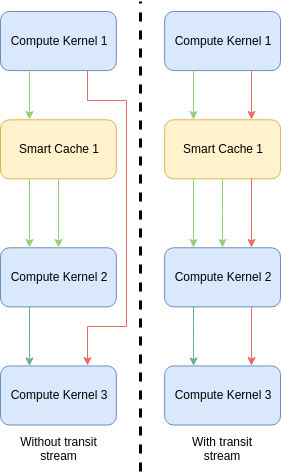
\includegraphics[scale=0.6]{images/Transit_stream.png}
    \caption{Example pipeline with and without transit streams}
    \label{fig:transit_stream}
\end{figure}

Figure \ref{fig:transit_stream} illustrates how transit streams affect a pipeline's layout, streams whose values have not changed are shown by arrows of the same colour. 
In the situation shown by Figure \ref{fig:transit_stream}, deadlock occurs in the version without transit streams as Compute Kernel 1 (CK1) will stop executing once it has written a value to the red stream connecting it to Compute Kernel 3 (CK3) and wait for CK3 to read that value. 
However, immediately after CK3 reads the value from CK1 it will block waiting to read a value from the blue stream connecting it to Compute Kernel 2.
This is problematic because the value of the blue stream is dependent on two values from the green stream which are supplied by Smart Cache 1.
The two values may be produced hundreds of driver loop iterations apart, meaning CK2 has to wait hundreds of iterations before it can begin executing. 
At this point, CK1 is free to write another value to the red stream to CK3 but this time it will not be read, as CK3 is still waiting for blue stream values from CK2, which in turn will not be able to execute as it is waiting for SC1's buffers to fill up (allowing SC1 to begin producing the required pairs of green stream values).
The pipeline is now deadlocked and execution grinds to a halt.
In the version with transit streams the red stream is passed through the SC1 meaning CK1 can output as many red values as it can green values.
This allows CK2 to start executing once the SC1 has filled up. 
CK2 now produces two synchronised output streams which CK3 can use as input.
Wherever a transit stream is found to be required, one is added as a \texttt{TransitStream} to the the list of input/output streams belonging to the appropriate \texttt{Kernel} objects.    

The next two compiler passes focus on inferring all the data required to synthesise the smart cache and memory access kernels needed by the compute kernels that form the pipeline.
The smart cache insertion pass runs first.
The goal of this pass is to replace any \texttt{StencilStream} inputs to a kernel with plain \texttt{Stream} inputs.
The compiler then iterates through the kernels in the pipeline and for each kernel with \texttt{StencilStream} inputs it analyses them in order to produce an appropriate smart cache to proceed the kernel in the pipeline. 
To generate a smart cache similar to the type introduced in \cite{VanderbauwhedeNabi2018}, the following data points must be gathered for each \texttt{StencilStream}:

    \begin{enumerate}
    \item The input stream.
    \item The size of buffer required to hold a window of the stream, large enough so that all the required stencil points can be produced.
    \item A list of output streams and which buffer index they are to be drawn from.
    \item The distances from the origin stencil point (effectively array index \texttt{X(i,j)}) to the stencil point furthest behind it and furthest in front of it (maximum negative and positive offset).
\end{enumerate}

All these data points can be gathered by counting the number array elements that occur between various combinations of the stencil points contained within the \texttt{StencilStream}.
The number of elements between two stencil points can be calculated using the dimensions of the array of which a stream is based.
The size of the smart cache can calculated by computing the number of elements between all pairs of stencil points and selecting the maximum value.
The maximum negative and positive offsets can be calculated by finding the largest distance between all pairs of points in which \texttt{(0,0,0)} appears as the first or second element in the pair respectively.
Finally, the buffer offset from which a smart cache output stream is to be read can be calculated as the number of elements from the first stencil point (first item of the pair used to calculate the required buffer size) and the stencil point itself.

\begin{figure}
    \centering
    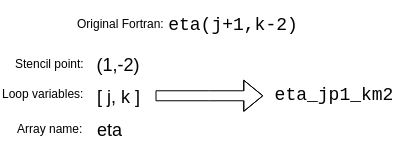
\includegraphics[scale=0.5]{images/rename_transform.png}
    \caption{Smart cache output stream name creation}
    \label{fig:stream_name_transform}
\end{figure}

Unique names for each of smart cache output streams can be derived by performing the transformation shown in Figure \ref{fig:stream_name_transform}.
This simple syntactic transform eases the scalarization pass described later in this section.
The input \texttt{Stream} for a smart cache can be created based on the original \texttt{Stencil\\Stream} input to the kernel. 

In order to prevent producing a pipeline which deadlocks, while also minimising the usage of the FPGAs limited on-chip block RAMs, a careful analysis has to be performed to decide which streams need to traverse a pipeline stage's smart cache.
Figure \ref{fig:smart_cache_stream_routing} illustrates the decision process used to decide whether a stream is to be added to the pipeline stages smart cache or not. 
As the flow diagram demonstrates, additional streams will often need to be buffered by a smart cache along side any \texttt{StencilStream} inputs.
It is usually necessary to route \texttt{TransitStream} and \texttt{Stream} inputs through the smart cache proceeding a compute kernel in order to keep their values synchronised with any \texttt{StencilStream} inputs derived by the smart cache.
If no streams are required to traverse a smart cache one will not be added to the pipeline stage.

\begin{figure}
    \centering
    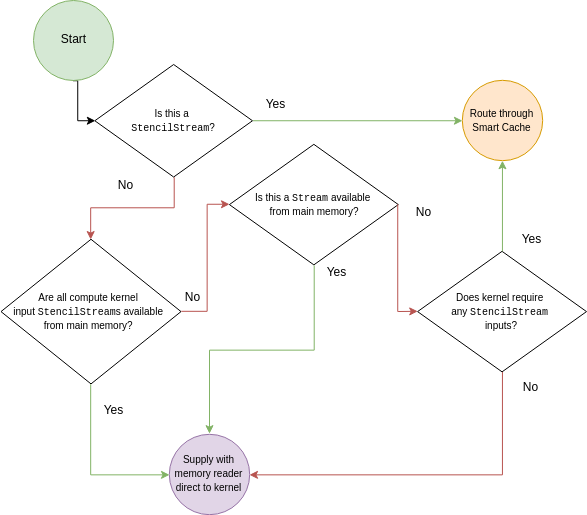
\includegraphics[scale=0.40]{images/Smart_cache_stream_routing.png}
    \caption{Decision process for deciding where compute kernel input streams come from}
    \label{fig:smart_cache_stream_routing}
\end{figure}

Once all the the streams required to pass through a smart cache have been identified, the data points are calculated for each of the \texttt{StencilStream} inputs.
The results from this analysis are then combined to find values for the smart cache as a whole.
The largest values for buffer size, maximum positive offset and maximum negative offset among all the processed \texttt{StencilStream} items are selected to be the values used for the smart cache as a whole.
This combination process is required as all the buffers within a smart cache must be the same size to prevent deadlocks.
Therefore, all the individual smart cache items must have their required buffer size padded to match the largest buffer size present in a smart cache.
To maintain correctness, the buffer offsets at which each output stream is drawn from must be updated to reflect the updated size of the buffer.
The value to be added to the original offset is simply the difference between the original buffer size and new buffer size.
At this point the parameters of the smart cache are fixed, so smart cache items can be generated for any non stencil streams that must also transit the smart cache.
These smart cache items only read one item from the buffer at the origin index, but are essential to keep the associated compute kernel's \texttt{StencilStream} and \texttt{Stream}/\texttt{TransitStream} inputs in sync.
Finally, once the smart cache associated with a compute kernel has had all its parameters calculated, the compiler is able to replace any \texttt{StencilStream} inputs to the compute kernel with the appropriate set of \texttt{Stream} outputs produced by the smart cache. 
Any smart cache outputs that come from a \texttt{TransitStream} or a \texttt{Stream} have the same name as the input stream.
Therefore, nothing needs to updated in the compute kernel's input stream list.
With this process complete, the compute kernel will only require normal input streams, which can be represented directly using OpenCL pipes. 

With the compute kernel now only requiring simple input streams, any memory access kernels necessary to allow the pipeline to read from and write back to the FPGA's main memory can be inserted.
Two types of memory access kernel are generated by F4 - memory reader kernels and memory writer kernels.
Memory reader kernels accept one parameter array only and simply loop over the array, emitting the values that make up the array one by one to their output streams.
These streams can then be consumed by a smart cache kernel or directly by a compute kernel.
% \footnote{It is important to note that although a memory reader kernel connected directly to a compute kernel may seem to be directly accessing main memory it is not the same as performing random accesses, as is required when using stencils. As such, there is no significant performance overhead.}. 
Conversely, memory writer kernels accept $N$ parameter arrays and loop over them writing the values they read from their input streams. 
The main task of the compiler, when generating memory access kernels, is deciding where to put them. 
For memory writer kernels this is easy.
The compiler simply walks to the last compute kernel in the pipeline and generates metadata for a memory writer suitable for writing all the kernel's output streams back to the appropriate arrays in the FPGA's main memory.
However, for memory readers the process is slightly more complicated. 
At this point the compiler begins to work with pipeline stages\footnote{A pipeline stage is defined as a compute kernel, a smart cache if one is required and any memory access kernels connected directly to either.} rather than just compute kernels.
A pipeline stage always contains a compute kernel and may contain a smart cache kernel; both of which may require an input stream from main memory.
The memory reader addition analysis performs a traversal of the pipeline comparing the inputs required by the kernels (compute and smart cache) making up that stage of the pipeline and the outputs available from the previous stage of the pipeline.
If any mismatch is found between the input streams required by the current stage and available output streams from the previous stage, a memory reader kernel is produced to output a stream of the value required.
This process highlights another reason for adding transit streams earlier during the compilation process.
All streams that have had their values modified or created within the pipeline, need to be present at all the intervening kernels between the produced and consumer kernels.
If transit streams were not added, any kernel requiring an input produced within the pipeline, but not by the kernel directly before it, would have a memory reader output to supply the input value as there would be a mismatch. 
This is undesirable, as it would result in incorrect values being output by the pipeline because later computations are performed using the original value of a stream.
If the stream is produced within the pipeline, the generated code would be invalid because the stream is ephemeral and not stored in memory. 
After memory access kernels are added all the compute kernels and the infrastructure necessary for their execution is in place, and the separate stages that make up the pipeline are complete. 

The final data-flow analysis step performed by F4 is designed to connect all the pipeline stages, and the components that make them up.
The goal of this step is to determine how many OpenCL pipes need to be created during the code generation phase and what pipes each kernel needs to read and write. 

The analysis works on a stage-by-stage basis. 
The basic idea of this pass is to match input and output streams and create a pipe object that can be attached to both the source and sink kernels allowing for the appropriate read and write calls to be output.  
Again, the pipeline is walked a stage at a time, any outputs from the previous stage are listed as a stage is being processed.
The process starts by building a list of pairs for each available stream.
the pairs consist of the stream and the source kernel that produces it.
In general this will consist of; any output streams from the previous stage's compute kernel, outputs from the current stage's smart cache (if one is required), and outputs from any memory readers (if it is the first stage in a pipeline there will obviously be no previous stage outputs available).
Next, a list of all the required streams and the kernel which needs them is built up, this will include; inputs to smart caches, inputs to compute kernels, and if this is the last pipeline stage, inputs to the memory writer. 
A map is then formed using the list of available streams and their sources.
The map entries are formed by grouping the list of available pairs by stream name.
The stream name common within a group is then used as the key and the group itself is used as the value.
The list of tuples pairing kernel's and one of their required input streams can now be iterated through, with the name of the required stream being used to look up the list of sources of that stream in the previously constructed map. 
The list returned from the map, contains all the kernels from which the consumer kernel can draw its input from.
From this list one item must be selected, enabling a pipe to be created connecting the producer and consumer kernel.
The selection process begins by filtering out any tuples where the source kernel is the same as the destination kernel.
For example, a smart cache will often output a stream with the same name as the input stream it accepts.
Obviously it would be incorrect to form a loop from the output of a smart cache back to its input.
Therefore, the list returned from this filtering operation is then sorted using a series of custom functions that take two potential sources and return a Haskell \texttt{Ordering}.
An ordering function is defined for each class of destination kernel (e.g. compute kernel, smart cache or memory writer) as they have different precedence rules where they get their input from. 
These functions can then be used with Haskell's \texttt{sortBy} function to rank all the potential producers for the consumer kernel.
One case that cannot be handled by this ranking technique arises when trying to connect a memory writer kernel and the compute kernel within that pipeline stage.
It is possible that outputs from the previous stage's compute kernel can have the same name as the outputs from the current compute kernel. 
This can lead to pipes being created linking the penultimate compute kernel to the pipeline's memory writer bypassing the final compute kernel.
This can easily be solved by comparing the pipeline stage order number attribute of all the potential source items for a stream.
If the destination kernel is a memory writer, any source kernels with a lower pipeline stage order than the destination can be filtered out. 
This removes any streams emanating from the previous stage's compute kernel.
Once these have been removed the usual ranking process can be used to produce the desired results.
Now that a source kernel has been chosen for the stream required by the destination kernel, a \texttt{Pipe} object is then generated. 
A \texttt{Pipe} object simply consists of the name of the OpenCL pipe to be generated (formed by concatenating the source kernel name, the destination kernel name and the stream name), the value type of the stream between the two kernels and the name of the stream. 
The generated \texttt{Pipe} is then added to the \texttt{readPipes} and \texttt{writtenPipes} lists of the destination and source respectively.

\subsubsection*{Scalarization}
\label{scalarization}

The final refactoring step aims to replace any array accesses that exist in the code that makes up a compute kernel with appropriately name scalar variables which can have their values read from and written to pipes. 
This pass works in a very similar way to the process used to generate the names of any output streams produced by a smart cache (illustrated in Figure \ref{fig:stream_name_transform}).
This time however, the index expressions used in an array access are converted to \texttt{<loop var name>(m/p)<offset value>} form directly, rather than to a stencil index first.
Each created index term is appended along with an underscore to the array name in the order they are used.

By performing the same transformation here as is performed when generating the smart caches, we can be sure the correct values will be used in the correct operations at run time. 
This also makes final code generation easier, as the stream name associated with any pipe objects can be used as the name of the written/read variable.

After any array accesses have be replaced by an appropriate scalar variable the last task is to complete an update of the compute kernel's argument and declaration lists.
This requires removing arguments and declarations associated with the original array accesses, and adding any declarations necessary to make the source code valid in light of the replacements of the arrays with scalar variables.  


\subsection{Code Emission}

The final compile process carried out by F4 is code generation.
During this step all the information collected by other parts of the compilation process is combined, and used to build a Fortran-style device code module.
This can then be converted to standard OpenCL C by RF4A, and from there synthesised to an FPGA bitstream using vendor specific HLS tools.
Code generation is handled a pipeline stage at a time.
First any required memory readers are generated, then (if required) the smart cache is produced, next the compute kernel itself and lastly a memory writer (if this is the last stage of the pipeline).

To ease the code generation process a small domain specific language (DSL) was created, this allowed AST nodes to be created easily from Haskell code.
Listing \ref{lst:dsl_examples}, provides two examples of how this DSL can be used to streamline the code generation system.
As the DSL simply builds \textit{language-fortran} AST nodes, they can be easily integrated with any existing code.
This proved very useful when generating the final kernel code for the compute kernels, as described below.


To generate the code for memory reader kernels the compiler simply emits a subroutine which takes one array argument.
The body is made up of a loop nest with the same number of loops as the number of dimensions the array has, bounded so that they cover all the items of the array. 
The body of the inner loop simply assigns the value found at the current index values from the array to a variable named after the stream name. 
The variable is then used to write to the memory reader's output pipe.

Memory writers work in a similar manner but can have multiple array arguments, however, it is required that all the arrays to be written have the same dimensions. 
A loop nest similar to that generated for memory readers is created and for each input stream a pair of statements is generated.
Firstly a pipe read call is added to read the appropriate input pipe into a variable named after the stream the pipe carries.
Then, an assignment statement is generated which writes the value read from the input pipe to the correct location in the main memory array using the loop indices.

Smart cache kernels are generated using exactly the pattern laid out in \cite{VanderbauwhedeNabi2018}.
The kernel's body consist of a driver loop that loops from 1 to the detected driver loop size + the maximum positive offset.
The maximum positive offset is added to the driver loop size to ensure the smart cache keeps emitting any values left in its buffers after it has stopped receiving input values.
Within the body of the driver loop is another loop that implements a left shift, moving all the buffer items one place to the left with the first buffer item being discarded. 
This leaves the first element of the buffer empty.
This can then be populated with the next value read from the appropriate input pipe.
Next, is a guarded section containing a pair of statements for each stream buffered by the smart cache. 
First the value from the input stream is read into a temporary variable, which is then assigned to the last position of the buffer array.
The section is guarded by an \texttt{if} that ensures it only gets executed while the driver loop is covering indices within the range 1 to driver loop size.
This prevents deadlocking caused by trying to read the input pipes after the kernels that write to them have stopped executing, but allows the smart cache buffers to empty allowing any kernels after the smart cache to complete their execution. 
The final section of the driver loop body is also guarded, as it is responsible for emitting the values from the smart cache and on to the compute kernel. 
This guard is designed to prevent the smart cache emitting values before the buffer has filled enough.
This would cause uninitialised values to be sent to the compute kernel, producing invalid results. 
In the write section, the buffer offset to output stream name tuples are used to read the appropriate location from the buffer and write it to the appropriate output pipe.
Statements of the form outlined above are output for each stream that needs to be buffered by the smart cache (using the data that was collected in the smart cache generation pass).

Code generation for the compute kernels works slightly differently than for the other kernels as some of the code exists already.
Firstly, any metadata (\texttt{OpenCLMap}/\texttt{OpenCLReduce}/ \texttt{OpenCLStencil} nodes) added by previous stages of the compiler are removed.
This leaves just the true Fortran code that makes up the kernel body.
Then calls to read the kernel's input pipes and write to the kernel's output pipes are generated.
Pipe read and write generation is straightforward as the name of the variable to read the pipe's value into/write the updated value to is attached to the pipe objects. 
Statements to read all the input pipes are generated and placed ahead of the subroutine body and statements to write any results to the appropriate output streams are generated and placed after the subroutine body.
Finally, the driver loop is generated using the data detected for the pipeline that the kernel belongs to. 
In the case of a map compute kernel one driver loop is inserted.
This contains the subroutine body sandwiched between the pipe-read statements and the pipe-write statements. 
However, in the case of a reduce kernel, two adjacent driver loops are emitted; one to perform the aggregation computation using the pipe-read block and the subroutine body.
This is followed by the second driver loop containing the pipe-write block, which produces a stream of the aggregated value.   
A subroutine is formed with its body only containing the driver loop. Its argument and declarations lists come from original compute kernel subroutine. 

The final step of the code generation process is responsible for outputting all the pipe declarations required to make the pipeline operational.
OpenCL pipes are declared using the \texttt{pipe} keyword, specific to OpenCL C.
As F4 generates a Fortran-syntax device module, and the goal was to generate syntactically valid output, a way was needed to declare pipes without the \texttt{pipe} keyword.
The following scheme was devised in collaboration with Dr W. Vanderbuawhede (developer of RF4A):

\begin{enumerate}
    \item At the module level a series of integer declarations were output, one for each required pipe. The name of the integer declarations for a pipe is the same as the \texttt{pipe} object's name will be in the final OpenCL C source.
    \item In addition to the kernel subroutines that make up a pipeline, the output device module would also contain a subroutine called \texttt{pipe\_initialisation}. For each pipe declared as an integer at the module level, \texttt{pipe\_initialisation} would contain a call to one of two artificial methods. These artificial methods named \texttt{ocl\_pipe\_real} and \texttt{ocl\_pipe\_int} accept a pipe as an argument, and are used as a hook by RF4A to determine that a module level integer declaration actually represents a pipe and the type of pipe it represents, thus allowing appropriate OpenCL C pipe declarations to be output. 
\end{enumerate}

\section{Evaluation}

The effectiveness of the F4 compiler is evaluated based on the output it produces when compiling tworeal world simulation systems - the 2D Shallow Water Model (2DSWM) \cite{Hall2009} and the Large Eddy Simulator (LES) \cite{Nakayama2011}.
Qualitative data characterising the compilation output is presented for both systems. 
The 2DSW model output generated by F4 is also evaluated empirically.
To do this the output from F4 is transpiled to OpenCL C using RF4A, this is then used to synthesise an FPGA bitstream using the vendor's HLS compiler toolchain. 
Output is compared to a version adapted for FPGA execution by a human expert (also synthesised using the same vendor toolchain), and assessed in terms of execution performance and FPGA resource consumption. 
Qualitative data for a hand translated version of the 2DSWM is also presented to allow more thorough comparisons to be made.
F4's output for the LES could not be tested on an FPGA device because the LES features circular boundary conditions. 
With the smart cache implementation that is currently used by F4 this type of boundary condition requires the entire stream to be buffered before the smart cache can begin emitting values (see Section \ref{data_flow_analysis_and_support_kernel_generation}).
This would lead to the smart cache's memory requirements dwarfing the amount of on-chip block RAM that an FPGA has available, and therefore HLS tools would not be able to synthesis a bitstream. 
However, this is not a fundamental limitation and with a more advanced smart cache implementation (which has already been developed \cite{Nabi2019}) this problem can be overcome.
Therefore, it is essential that F4 can handle code bases that feature these types of boundary conditions so that in future work a more advanced smart cache implementation can replace the current implementation. 
The F4 compiled version of the 2DSWM has been executed on an FPGA and its output results have been validated against the output from the original Fortran implementation, as has the hand translated version.

The input code bases used in this evaluation have been preprocessed by RF4A as described in Section \ref{parsing}.
The exact versions of the code bases used in this evaluation can be found in the project repository. 

\begin{table*}[]
\begin{tabular}{c|c|c|c|c|c|c}
\textbf{System}                                                   & \textbf{Pipeline ID} & \textbf{Compute Kernels} & \textbf{Smart  Caches} & \textbf{Memory Readers} & \textbf{\begin{tabular}[c]{@{}c@{}}Memory \\ Writers\end{tabular}} & \textbf{Pipes} \\ \hline
\begin{tabular}[c]{@{}c@{}}2DSWM \\ (F4 Compiled)\end{tabular}    & 0                                                               & 5                                                                   & 4                                                                & 16                                                                 & 1                                                                  & 58             \\ \hline
\begin{tabular}[c]{@{}c@{}}2DSWM\\ (Hand Translated)\end{tabular} & 0                                                               & 4                                                                   & 3                                                                & 1                                                                  & 1                                                                  & 71             \\ \hline
LES                                                               & 0                                                               & 12                                                                  & 8                                                                & 70                                                                 & 1                                                                  & 269            \\
                                                                  & 1                                                               & 1                                                                   & 1                                                                & 6                                                                  & 1                                                                  & 28             \\
                                                                  & 2                                                               & 5                                                                   & 3                                                                & 5                                                                  & 1                                                                  & 17            
\end{tabular}
\caption{OpenCL pipelines component breakdown}
\label{pipeline_components}
\end{table*}

Table \ref{pipeline_components} provides a breakdown of the components that make up the various device modules. 
It shows the the number of pipelines a system has been broken into as well as the components that make up each pipeline.
The data shows that the 2DSWM only requires one pipeline, whereas the LES requires three. 
This is the expected result in both cases.
All the loop nests in the 2DSWM are of the same depth so a single pipeline is possible without wasting execution cycles.
In this respect F4's output mirrors the layout of the hand-translated version of the 2DSWM.
For the LES 3 pipelines is also the expected result. 
When inspecting the codebase, it becomes clear that the 1 kernel pipeline with ID 1 corresponds to the successive-over-relaxation (SOR) loop nest found in the press subroutine. 
In this section of code, the array traversal loop nest found throughout the LES, is itself enclosed in an additional loop which performs 50 iterations.
The entire array is traversed 50 times during this section's execution.
This dramatically increases the total number of iterations required when compared to adjacent loop nests.
Therefore, F4 has correctly allocated it to its own pipeline, causing a split and leading to a total of 3 pipelines being produced. 
The pipelines with IDs 0 and 2 only contain loop nests 3 loops deep.
If the SOR loop nest is omitted the LES can be handled in one pipeline.
These results show the pipeline detection pass of the compiler works and produces valid pipelines. 
Unfortunately, as the LES output could not be synthesised to hardware, more stringent tests could not be performed. 

\begin{figure}
    \centering
    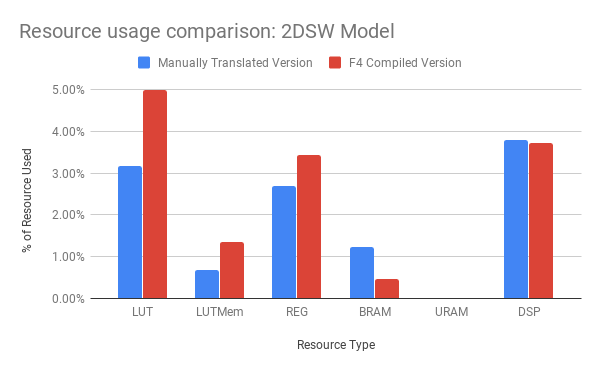
\includegraphics[scale=0.4]{images/Resource_usage_comparison_2DSW_Model.png}
    \caption{2DSWM resource usage comparison}
    \label{fig:resource_usage}
\end{figure}

The F4 compiled version of the 2DSWM is now compared with the version produced by a human expert \cite{VanderbauwhedeNabi2018}. 
First the implementations are compared in terms of resource usage.
Figure \ref{fig:resource_usage} shows the percentage of the FPGA's resources that have been consumed by each implementation.
The results are broken down into 6 categories. 
The data presented here is produced by Xilinx's HLS toolchain when synthesising a bitstream for one of their Ultrascale+ 16nm VU9P FPGAs.
These FPGAs can be accessed through Amazon Web Services using an F1 EC2 instances.
The results show that the compiler output uses more lookup table (LUT) and register resources but fewer block RAMs and DSPs.
This result is expected as the most significant difference between the compiler generated code and the hand translated code is their approach to reading streams from memory.
As Table \ref{pipeline_components} highlights, the hand-translated version uses 1 memory reader, whereas the compiler generated pipeline uses 16.
The memory reader is placed at the start of the pipeline in the hand translated version.
It reads all the input arrays in order to produce all the streams required as input by every kernel in the pipeline. 
The outputs from this memory reader are then passed through all the intervening smart caches and compute kernels to where they are required as inputs. 
As described in Section \ref{data_flow_analysis_and_support_kernel_generation}, the approach taken by F4 is to output one memory reader per stream, and have them directly connected to the kernel that requires the stream as input.
The difference between these approaches largely explains the discrepancy between the resource usages shown in Figure \ref{fig:resource_usage}.

Increasing the number of memory readers is expected to increase the usage of LUTs and registers as there is redundancy.
Multiple memory readers can be emitted for the same input array at different stages of the pipeline.
However, as expected, increasing the number of memory readers leads to a reduction in block RAM usage as fewer streams need to be passed through a pipeline's smart caches in order to keep them synchronised.  
This trade-off is likely to be desirable as block RAMs are usually the scarcest resource available on an FPGA.
Further, the magnitude of the increase in LUT/register usage, when taking F4's approach, is less than the magnitude of the decrease in block RAM usage. 
The approach taken by the compiler is therefore likely to scale more readily.

% However, additional memory readers are not the only cause of increases in LUT and register usage.
% In the F4 compiled device module, 5 compute kernels are produced compared to 4 in the hand-translated version.
% This is a result of the human expert's intuition that the \texttt{dyn\_0} and \texttt{dyn\_1} kernels from F4's output can be merged to produce a single \texttt{dyn\_1} kernel. 
% Figure \ref{fig:kernel_alloc} compares the resource usage for the two compute kernels produced by F4 (blue and red bars), with the resource usage for the single kernel developed by the human expert (orange bar).
% As Figure \ref{fig:kernel_alloc} illustrates, LUT and register usage is higher in the two kernel solution than it is for the one kernel solution.
% As the compute logic for both solutions is the same, this discrepancy illustrates the overhead that comes from using multiple kernels. 
% This could be a target for optimisation in further work and could lead to a narrowing of the LUT and register usage gap between F4's output and code produced by a human expert, while still retaining the benefit of reduced block RAM usage.
% 
% \begin{figure}
%     \centering
%     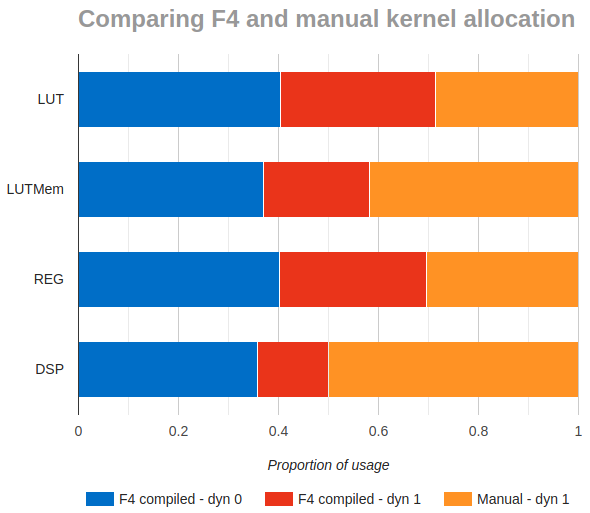
\includegraphics[scale=0.30]{images/Comparing_F4_and_manual_kernel_allocation.png}
%     \caption{Kernel allocation's effect on resource usage}
%     \label{fig:kernel_alloc}
% \end{figure}

\subsection{Performance Evaluation}
\label{perf_eval}

Unfortunately, due to time constraints the Xilinx FPGA could not be used to test the execution performance of the compiled bitstream.
As a fallback, an Intel Stratix V D5 FPGA owned by the University of Glasgow, was used to gather performance data for the 2DSWM.
Version 15.1 of Intel's HLS tooling was used to synthesise a bitstream.
Again, due to time constraints generation of an OpenCL host module was not completed.  
Therefore, to run the synthesised bitstream on the FPGA a host module needed to be developed manually.
Dr W. Nabi kindly provided one, which was capable of executing both the F4 generated 2DSWM device module and the hand translated version.  
An Intel Xeon E5-2609 v2 CPU was used to execute the CPU baseline.
The CPU baseline was written in C++ and compiled with \texttt{g++} with optimisation level \texttt{-O3}.


\begin{figure}
    \centering
    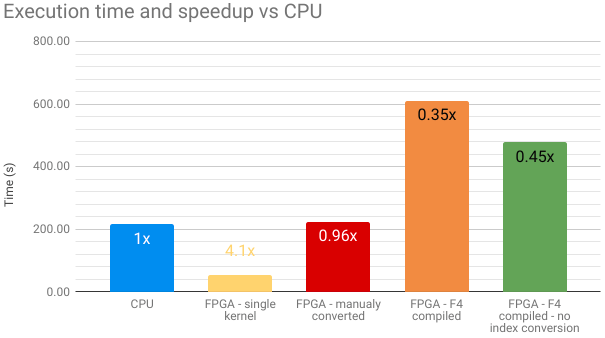
\includegraphics[scale=0.40]{images/Execution_Time_and_Speedup_vs_CPU.png}
    \caption{Execution times for 2DSWM over a 502 x 502 grid for 10,000 time steps, and speed up compared to CPU}
    \label{fig:exec_perf}
\end{figure}

Figure \ref{fig:exec_perf} shows the execution performance of the tested versions of the 2DSWM.
A naive single kernel OpenCL port of the 2DSWM was also bench marked to show the importance of correctly structuring code targeting FPGAs.
The timing data was gathered by running the 2DSWM for 10,000 time steps.
Each model was executed 4 times and the average of the 4 execution times was then computed. 
The execution performance data gathered was not as was expected.
The optimised FPGA code produced by the human expert and F4 performed significantly worse than the CPU baseline and the naive single kernel system.
Additionally, the code generated by F4 and RF4A performed far worse than all other versions of the code. 
A series of experiments were performed in order to determine areas for future optimisation. 
During these experiments, both the host code and device code were edited manually and results collected.
The first optimisation made was to pre-compute the conversions necessary to change the Fortran convention array accesses to C style.
This change did result in a speed up when compared to the original F4 output but it was still much slower than all the other versions. 
The next optimisation was to move the time loop which drives the simulation from the OpenCL host to the device code.
The aim was to significantly reduce the time lost to context switches between the device and the host. 
This optimisation was applied to all the OpenCL versions of the code to ensure a fair comparison.
The time loop was moved in conjunction with the array access convention optimisation for the F4 output.
The results for the code with the device time loop are shown alongside the CPU baseline in Figure \ref{fig:exec_perf_device_time_loop}.
The effect of this optimisation is dramatic. 
The pipelined FPGA code shows significant speed increases, with the human experts code running over 16x faster than the CPU baseline and nearly 4x faster than the single kernel port.
More importantly, the code generated by F4 is nearly 20x faster than the CPU baseline, and over 4.5x faster than the single kernel version.

\begin{figure}
    \centering
    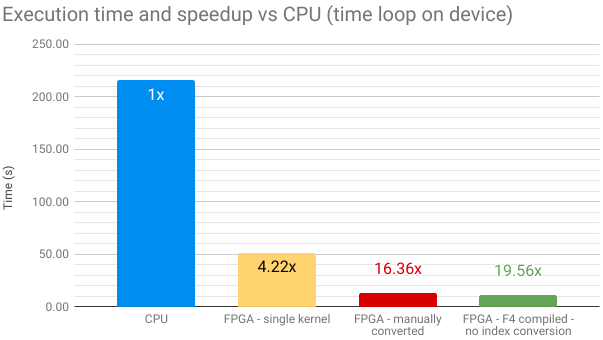
\includegraphics[scale=0.40]{images/Execution_Time_and_Speedup_vs_CPU_device_time_loop.png}
    \caption{Execution times for 2DSWM over a 502 x 502 grid for 10,000 time steps, and speed up compared to CPU - simulation time loop on FPGA}
    \label{fig:exec_perf_device_time_loop}
\end{figure}

\section{Conclusions and Future Work}

This paper presents a compiler capable of analysing Fortran code and refactoring it to produce a series of optimised OpenCL pipelines which can be executed using an FPGA. 
The compiler refactors array-based sequential code into stream-based code which can benefit from the pipeline parallelism that FPGAs offer. 
The compiler builds a streaming pipeline designed to optimise memory accesses. This has been shown to be essential for efficient execution on FPGAs \cite{VanderbauwhedeNabi2018}. 

The evaluation shows that the compiler can accept real world code bases as its input and produce an FPGA pipeline that outputs the same results as the original Fortran implementation.
Output from F4 was also compared to a system converted from Fortran to FPGA-optimised-OpenCL by a human expert.
This comparison demonstrated that the compiled code produced the correct results.
Additionally, with some minor alterations, the F4 generated code was shown to outperform all the tested versions of the 2DSWM.
A 20x speedup was achieved when compared to the same system executing on a CPU. 

F4 has been shown to accept real world legacy Fortran as input and produces an optimised, FPGA-ready solution, which outputs the same results as the original system. 
This allows systems written decades ago to benefit from cutting-edge advances in computer hardware, delivering performance improvements to their users - many of whom are working to solve the world's most important problems.

\subsection{Future Work}

The most pressing work to be performed on the F4 project is to implement the manual optimisations described in Section \ref{perf_eval}.
These optimisations are ``low-hanging fruit'' and, with collaboration from the authors of RF4A, can easily be implemented. 
Moving the time loop to the device links well with the next area requiring attention, namely having F4 produce a host module.
All the relevant metadata required to produce a host module is output alongside the device module.
Adding this functionality will be relatively simple. 
To get good performance from multi-kernel device modules, it is essential that the time loop is executed on the device, to reduce the device-host context switch overhead (as the results presented in Section \ref{perf_eval} show).
One complication is that OpenCL does not provide a set of Fortran host APIs.
A useful project which can be used in place of an official Fortran API, is OpenCLIntegration \cite{Vanderbauwhede2012}.

Another opportunity to extend this work would be to integrate the smart cache implementation capable of handling circular boundary conditions (described in \cite{Nabi2019}) with F4.
If this augmentation was completed, the output generated by F4 for the LES would be able to be synthesised and run on an FPGA.
This would allow further testing and validation of the output to be carried out.
The new smart cache design is implemented in Verilog, so would be difficult to integrate directly with the OpenCL currently produced by the compiler.
One way to solve this would be to more closely integrate F4 with some of the work being carried out as part of the TyTra project \cite{Nabi2015}.
If F4 had the capability to emit TyTra-IR it would be more flexible and would not run into many of the issues caused by using OpenCL as its route to hardware.

% Finally, and most simply, to reach the goal of providing a turnkey solution, it is essential to continue testing F4 with as wide a variety of real world code bases as possible. 
% By fixing bugs and mitigating against oversights that come to light during F4's use, it can be ensured that as many people as possible can benefit from the power offered by FPGAs.  


%\vspace*{\fill}

{\bf Acknowledgments.}
I would like to thank Dr W. Vanderbauwhede and Dr W. Nabi for their help and support during the course of this project. It has been a roller coaster!
%great challenge and truly interesting!

\clearpage
\appendix

\section{Code examples}

\begin{listing}[ht]
\inputminted{fortran}{snippets/stencil_constant_removal.f95}
\caption{Example of stencil computation before and after constant removal preprocessing pass.}
\label{lst:stencil_constant_removal}
\end{listing}

\begin{listing}[ht]
\inputminted{fortran}{snippets/stencil_detection.f95}
\caption{Result of stencil detection}
\label{lst:stencil_detection}
\end{listing}

\begin{listing}[ht]
\inputminted{fortran}{snippets/kernel_extraction.f95}
\caption{Example of extracted kernel}
\label{lst:extracted_kernel}
\end{listing}

\begin{listing}[ht]
\inputminted{fortran}{snippets/kernel_with_loop_guards.f95}
\caption{Kernel with guards and index derivation}
\label{lst:with_loop_guards}
\end{listing}

\begin{listing}[ht]
\inputminted{haskell}{snippets/fortran_dsl_examples.hs}
\caption{Examples of the Fortran DSL used during code generation}
\label{lst:dsl_examples}
\end{listing}

% Analysis to avoid transiting all streams when pipe buffer depth will all writes to continue
% 
% Smart cache buffers do not need to be the same size, could guard blocks in current shift loop or add multiple shift loops would have to see which was most efficient with space.
% 
% host code generation.
\clearpage
\bibliographystyle{abbrv}
\bibliography{main.bib}


\end{document}
